\chapter{Web Service clients}\label{chap:ws_clients}
A Web Service client is the consumer of a Web Service. According to
Definition~\ref{def:ws} the consumer can be any HTTP client at the other end of
the line, e.g., an Ajax client. In this chapter, we introduce what is probably
\textit{the} most popular style for Web Service clients: Ajax. Ajax is presented
in the light of REST, leaving important things behind, such as the
\verb|XMLHttpRequest| object. In addition, we introduce JSON; a simple data
format for interchanging data between servers and clients.

%and why JSON is chosen as representation
%format for the surf weather service.

%We discuss the advantages of a \textit{\gls{gls:fat_client}} approach for the
%user interface.
\section{Ajax: the style for modern Web Service clients}\label{sec:ajax}
Ajax is a style for a set of Web technologies that narrow the gap between the
``richness and responsiveness'' of desktop applications and Web applications
\citep{ajax:coined}. Initially, the technologies used in Ajax were incorporated in
the name itself. Ajax is short for Asynchronous JavaScript + XML; however, in
many newer Web applications the XML has been replaced by JSON.

In Ajax applications, an Ajax engine on the client side extends the HTTP
request-response cycle by communicating asynchronously with the
server. Traditionally, in server-side Web applications, a client's request result
in the server crafting and returning a unique HTML page to the user. The Ajax
style, however, allows for putting the logic of crafting the page on the
client\footnote{The Ajax style also allows for small page updates of a site
crafted at the server; this is, however, not the focus of this section.}, and
lets the server handle pure \textit{\gls{gls:business_logic}}. The approach has
the following advantages:
\begin{itemize}
  \item the server is relieved of compositioning Web pages;
  \item the presentation of data at the client is separated from the producer of
  it; and
  \item the Web application can be made more rich and responsive.
\end{itemize}
Most server-side applications that customize pages violate the REST style of
statelessness: \textit{\gls{gls:appstate}} is put on the server in order to
create customized pages effectively. Maybe the biggest advantage of the Ajax
style is that it can circumvent the problem of customization by placing
\gls{gls:appstate} where it belongs in terms of REST, in the client.

The benefits of the Ajax approach over a usual server-side approach are numerous:
\begin{itemize}
  \item it is possible to create dynamic customized sites with a stateless
server;
  \item static files, such as the Ajax client, are cached at the client after the
user's first access to the page, therefore, on additional requests only new
business data is loaded from the server. Compare this to a server-side approach
where a unique page is created for every user.
\item business data is isolated boosting cache hits on intermediate servers for
all clients. In addition, an optimal caching strategy for each type of component
can be applied. Compare this to a server-side strategy where any change in
the site must invalidate the cache.
\end{itemize}
Thus, an Ajax approach supports REST while at the same making customized Web
sites possible. Hereby the Ajax approach inherits one of the main quality
attributes of REST: scalability \citep[p.116]{rest:Fielding02}

The drawbacks of adopting the approach are that 1) the application needs to be
implemented using several languages: one for the server-side Web Service, and
JavaScript for the client-side; 2) clients need to have JavaScript enabled, and
3) JavaScript is the language of implementation making well-known Web application
frameworks -- and all their tools such as debugging tools -- useless for anything
else than creating Web Services.

%The Ajax client can consume data from different types of Web Services, e.g., Big
%Web Service or RESTful Web Services. Using a RESTful Web Service for serving
%data, however, gives all the advantages stated in the REST architectural styles overview
%in Table~\ref{tab:REST} now apply for the application.


\section{JSON}\label{sec:json}
JavaScript Object Notation (JSON) is a data interchange format. JSON is a subset
of JavaScript and described as ``The Fat-Free Alternative to XML''
\citep{json:fat-free} and indeed since its introduction Web developers and Web
Services have adopted JSON as the simpler and cleaner data interchange format
with companies such as Yahoo and Google embracing JSON
\citep{json:yahoo,json:google}. One of the reasons JSON is
widely adopted is due to its simplicity: the syntax can be described with a
context-free grammar in just a few lines:
\begin{verbatim}
  <Literal> ::= <Object> | <Array> | string_literal | numeral | 
                boolean_literal | null 
  <Object>  ::= {} | { string_literal: <Literal>} | 
                { <Object>, <Object>} 
  <Array>   ::= [] | [<Literal>] | [<Literal>, <Literal>]
\end{verbatim}
In addition, JSON is efficiently used within JavaScript, and JSON can circumvent
the same origin policy. A JSON response is de-serialized into JavaScript objects
by using the JavaScript \verb|eval()| function:
\begin{verbatim}
var data = eval('(' + json_response + ')');
\end{verbatim}
The \verb|eval()| function takes a string as parameter and evaluates it as if it
were JavaScript code directly written in the document. Since JSON is a subset of
JavaScript \citep{json:fat-free} JSON can be de-serialized with
\verb|eval|. However, that approach is subject to \textit{\gls{gls:xss}} if the
response contains user generated data. See Appendix~\ref{sec:xss} for an example
of using a raw eval to inject and execute JavaScript code. Instead of using eval
to de-serialize data we use a JSON parser\footnote{http://www.json.org/json2.js}.

\begin{figure}[htbp]
  \centering
  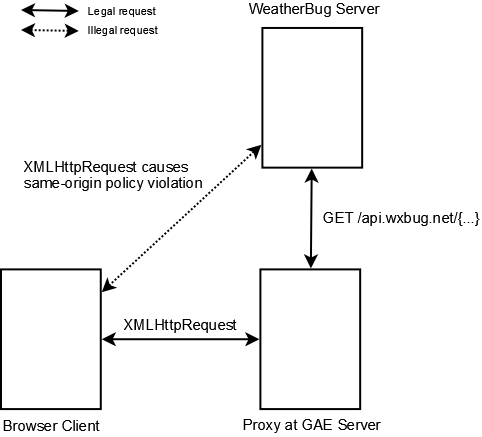
\includegraphics[scale=0.3]{./Figures/proxy}
  \caption{Circumventing the same origin policy with a proxy}
  \label{fig:proxy}
\end{figure}

The same origin policy is a set of security restrictions imposed by
browsers. They prohibit access to methods and properties of documents served from
other origins compared to the document where it is embedded. Origin is defined by
most browsers as the hostname and port number
\citep{browsersec:part2}. Therefore, e.g., external Ajax requests and Document
Object Model (\textit{\gls{gls:dom}}) access to external content in frames are
impossible: the content must stem from the same domain to do this.

A workaround to enable access to cross-domain data is setting up a proxy that
tunnels all request to a server at another domain through the server hosting the
current site. An example where we could have set up a proxy to circumvent the
problem is for XML weather data resources from WeatherBug. The resources are not
in JavaScript format which makes it impossible to load data directly from
WeatherBug into the client. Therefore we could setup a proxy that tunnels all
request to the WeatherBug API through the GAE server, as shown in
Figure~\ref{fig:proxy}.

Another reason for the success of JSON is due to an exception in the same origin
policy: it does not apply for externally valid JavaScript loaded via the HTML
\verb|<script>| tag. Script tags are untouched by the same origin policy, and
therefore many Web Services provide data in JSON format. Client access JSON
Web Service by dynamically creating \verb|<script>| tags and inserting them into
the document; upon insertion the browser fetches the external content into the
document. Now how do we know when that \verb|<script>| tag has finished loading?
If the Web Service is able to wrap the JSON object in a user-chosen function we
have JSONP \citep{json:defined}. With JSONP that user-defined function is called
automatically when the \verb|<script>| tag is loaded. 

\section{Summary}
In this brief chapter we introduced Ajax from a RESTful perspective, which
included an overview of the advantages of the Ajax style where the server is a
pure holder of business data.
